\chapter{Introducción}
\label{cap1}

A principios del siglo XX se descubrió la existencia de los rayos cósmicos. Estos son partículas subatómicas provenientes del espacio exterior. Estas
partículas, en su mayoría protones y núcleos de Helio son muy energéticas debido a su gran velocidad. El origen de estas no es muy claro, pero sabemos
que proceden del espacio exterior. Raras veces la actividad solar puede producir partículas tan energéticas. 
\par
Muchas de estas partículas inciden con la atmósfera terrestre. En las capas altas de la atmósfera se producen las primeras interacciones, estas
partículas colisionan con partículas que forman la atmósfera. Esta colisión es muy violenta y causa la división de las partículas originales en
partículas segundarias. Estas a su vez pueden colisionan con otras partículas de la atmósfera para así formar aún más partículas segundarias. Vemos
como una sola partícula proveniente del espacio produce el fenómeno denominado \emph{cascadas atmosféricas}. Como es de esperar con cada choque
consecutivo se pierde parte de la energía. Normalmente las partículas segundarias que alcanzan la superficie terrestre tan solo tienen una pequeña
fracción de la energía inicial. Si una partícula no posee la energía suficiente la cascada que es originada no se propaga hasta la superficie
terrestre.
\par
Como hemos dicho la mayor parte de la radiación cósmica proviene de fuera de nuestro sistema solar, pero está fuertemente relacionada con los ciclos
solares. Los ciclos solares de 11 años aproximadamente afectan la actividad solar pasando por un mínimo y un máximo, donde los cambios son apreciables
en la luminosidad y el campo magnético. Es este segundo, el campo magnético solar, el que afecta a la llegada de radiación cósmica a la Tierra. Al ser
mayormente partículas con carga eléctrica en la presencia de un fuerte campo magnético estas son desviadas. A continuación detallamos los sucesos más
comunes que pueden ser observados indirectamente a consecuencia de observar la cantidad de radiación cósmica.
\begin{itemize}
	\item	Ciclo solar. Como hemos explicado existe una fuerte relación entre la cantidad de radiación cósmica y la actividad solar. La radiación
		cósmica es un buen indicador de la actividad solar donde la relación es inversa. Menos radiación generalmente significa una actividad
		solar elevada.
	\item	Forbush decrease\cite{Forbush1938}. Estos sucesos consisten en un descenso rápido de los niveles de radiación cósmica medida en la
		Tierra. Estos descensos son consecuencia de CME's. La materia expulsada en un CME al ser en su mayoría plasma extiende e intensifica
		el campo magnético solar. Como ya hemos explicado el aumento del campo magnético solar conlleva al descenso de radiación cósmica.
	\item	Ground level enhancements. Eventualmente la actividad solar es tan elevada que el Sol es capaz de emitir partículas muy energéticas.
		Estas partículas son a veces tan energéticas que pueden generar cascadas atmosféricas que alcanzan la superficie terrestre. Estos
		sucesos son muy raros, entre 10 y 15 por década. A pesar de ser muy raros estos pueden tener un gran impacto en nuestras vidas
		cotidianas, pueden afectar el funcionamiento de la electrónica sensible que está en orbita e incluso la que está en tierra.   
\end{itemize}

\section{Monitor de neutrones}
	Un monitor de neutrones es una estación terrestre que monitoriza la llegada de partículas extraterrestres de forma indirecta a partir de las
	cascadas atmosféricas. Estos están compuestos por cuatro capas especialmente diseñadas para capturar las partículas segundarias producidas en
	las cascadas atmosféricas. A continuación procedemos a explicar estas cuatro capas, empezaremos por la más exterior y acabaremos explicando la
	capa más interior.
	\begin{itemize}
		\item	Reflector. La primera capa consiste en un escudo reflector que tan solo deja pasar las partículas con energías altas. De esta
			manera todas las partículas generadas por el entorno inmediato que tienen baja energía rebotan y no influyen en la medición.
		\item	Productor. Esta capa compuesta generalmente de material denso tiene como objetivo conseguir algo parecido a las cascadas
			atmosféricas. La idea es tener un material denso para que sea muy probable que las partículas secundarias impacten con las
			partículas del material y como resultado se produzcan aún más partículas. A las partículas generadas en esta capa se les da el
			nombre de neutrones de evaporación. Son estas partículas las que finalmente serán medidas por el instrumento, también son las
			que le dan nombre. Los neutrones producidos tienen menos energía, por lo que son más fáciles de medir.
		\item	Moderador. A pesar de que las partículas que tenemos a este nivel tienen tan solo una fracción de la energía original estas
			aún siguen siendo demasiado energéticas para ser capturadas. Esta capa tiene como objetivo relentizar, disminuir la energía,
			de las partículas para así poder capturarlas.
		\item	Contador. Un contador o tubo contador generalmente está relleno de gas ionizado con propiedades específicas. Cuando una de
			las partículas relentizadas por el Moderador choca con una de las partículas del gas es liberada una pequeña cantidad de
			energía en forma de electricidad, una señal eléctrica que podemos medir. 
	\end{itemize}
	\par
	Los sistemas de adquisición están diseñados para recoger estas pequeñas señales y medirlas. Tradicionalmente la medida que se realiza son
	eventos por minuto, las señales son capturadas, amplificadas y registradas en un contador que se reinicia cada minuto. A lo largo de este
	trabajo muchas veces nos referiremos a esta medición de eventos por minuto con el nombre de \emph{cuentas}. 

\section{NMDB}
	NMDB\cite{NMDB2011} o \emph{Neutron Monitor Database} es una red mundial de monitores de neutrones. Antes de proceder a hablar sobre la red
	en concreto expondremos las ventajas y razones de una red como esta.
	\begin{itemize}
		\item 	Espectro de energías. Al igual que el Sol, la Tierra tiene campo magnético. Este campo magnético repele con mayor fuerza en
		  	las regiones ecuatoriales que en los polos. Esto implica que solo las partículas más energéticas son perceptibles en las
			zonas ecuatoriales, mientras que en los polos las partículas no necesitan ser tan energéticas para alcanzar la superficie.
			Combinando dados de estaciones que se encuentran a diferentes latitudes podemos construir espectrogramas basados en la energía
			de las partículas.
		\item 	Anisotropía. Tener estaciones en diferentes lugares del globo terráqueo implica estar orientado a diferente dirección del
		  	espacio. Esto implica poder realizar estudios sobre la procedencia de eventos.
		\item 	Redundancia. Tener muchas estaciones implica detectar el mismo evento en más de una estación. Esto permite comparar los datos
		  	entre estaciones y descartar fluctuaciones grandes, rápidas y asiladas en una sola estación.
		\item 	Cooperación. Estar en una red implica mejorar la comunicación entre las diferentes estaciones. De esta manera los resultados
		  	son mejores y el avance más rápido. 
	\end{itemize}
	\par
	Como ya hemos comentado NMDB es una red mundial, impulsada por la Comisión Europea. Actualmente la red supera las veinte estaciones. La red
	proporciona datos en tiempo real con resolución de un minuto. Los formatos de los datos están estandarizados entre las diferentes estaciones,
	esto ayuda al análisis científico de estos. Los datos en tiempo real son utilizados para la elaboración de un sistema de alarma
	GLE\cite{GleAlarm}. Como hemos explicado un GLE fuerte puede tener un impacto grande en nuestras vidas diarias, un impacto negativo. Es
	interesante poder detectar estos eventos lo antes posible, este es uno de los objetivos principales del NMDB. 

\section{CALMA}
	CALMA\cite{Medina2013} o \emph{Castilla la Mancha Neutron Monitor} es el primer y único monitor de neutrones en España. Este forma parte del
	NMDB, el equipo técnico responsable de la estación está profundamente implicado en desarrollar sistemas y herramientas que mejoran la red. Un
	ejemplo es el sistema de adquisición implantado en la estación, también implantado en otras estaciones de la red. La estación empezó a operar
	de forma plena en diciembre de 2012 y desde entonces lleva haciéndolo ininterrumpidamente con pequeñas excepciones. Desde su puesta en marcha
	la estación ha registrado 18 Forbush decreases. Desafortunadamente aún no ha habido ningún GLE que detectar, aunque este tendría que ser muy
	energético para ser detectado en una estación con tan poca latitud. A continuación procedemos a hablar más a fondo del estado actual de CALMA,
	hablaremos del sistema de adquisición, base de datos, herramientas y técnicas que son usadas.
	\subsection{Sistema de adquisición}
		Como hemos mencionado el sistema de adquisición que está implantado en CALMA es producto del propio equipo\cite{Garcia2014}. El
		sistema es basado en un sistema empotrado Linux. Las señales capturadas por los tubos contadores son amplificadas y digitalizadas por
		un circuito de adaptación, seguidamente son procesadas por una FPGA. Esta es la encargada se medir los eventos por minuto de los 18
		canales. Aunque la  estación tan solo tiene 15 tubos contadores el sistema está diseñado para soportar 18, este número es un estándar
		histórico. El software que se ejecuta en el sistema Linux tiene como tarea comunicarse con la FPGA, su labor es recoger las
		\emph{cuentas} de cada minuto y guardar estas en una base de datos. En la figura \ref{fig:acqsis} podemos ver que diagrama de bloques
		que representa el sistema de adquisición.
		\begin{figure}[h]
			\centering
			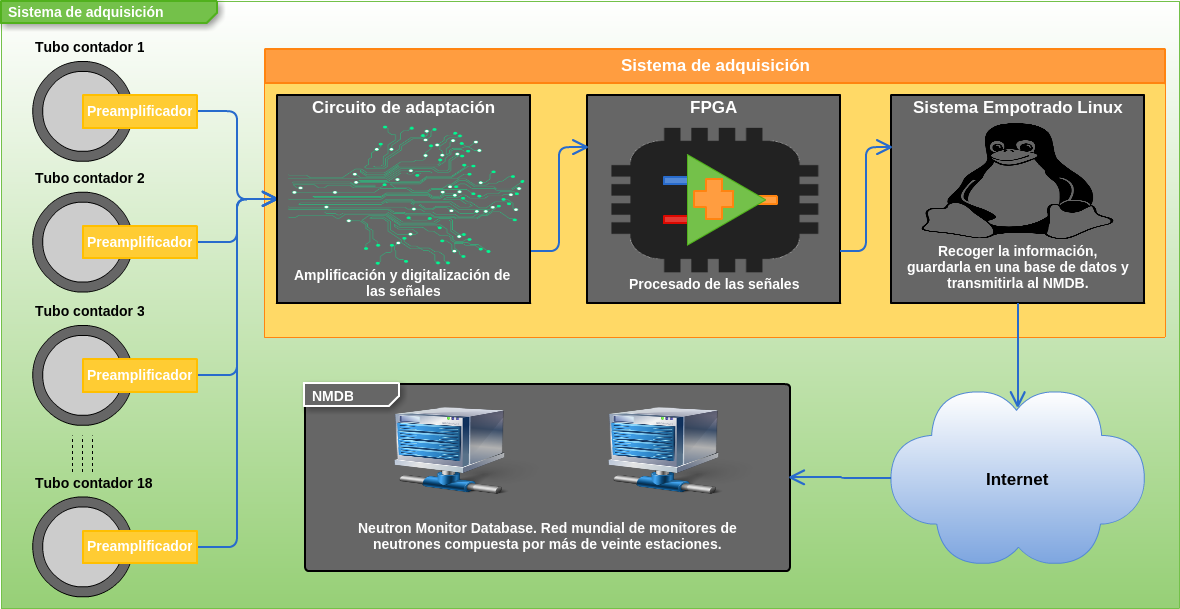
\includegraphics[keepaspectratio, width=1\textwidth]{./img/AcqSis.png}
			\caption{Sistema de adquisición.}
			\label{fig:acqsis}
		\end{figure}
		\par
		Actualmente el equipo de CALMA está desarrollando un nuevo sistema de adquisición de datos. Este es muy parecido al que actualmente
		está implantado. A continuación procedemos a detallar las diferencias clave entre los dos sistemas. 
		\par
		\begin{itemize}
			\item La primera diferencia entre los dos sistema de adquisición radica en el circuito de adaptación. En el sistema de
			  adquisición actual para cada señal el circuito de adaptación genera un pulso fijo. El nuevo sistema de adquisición incorpora
			  nuevo circuito de adaptación. Este nuevo circuito de adaptación genera un pulso cuyo ancho de banda es proporcional a la
			  energía de la señal. El fin es medir la energía de las partículas detectadas, esta magnitud es de gran interés científico y
			  técnico.
			\item La siguiente diferencia está en la FPGA, recordamos que en el sistema de adquisición actual esta tan solo registra los
			  eventos por minuto para los 18 canales. La nueva FPGA debe realizar la misma tarea, pero aparte debe poder medir el ancho de
			  los pulsos generados por el circuito de adaptación. Los dos sistemas de adquisición utilizan un puerto serie para la
			  comunicación entre software y FPGA, en el sistema nuevo este puerto opera a una velocidad mayor a fin de poder transmitir
			  toda la información extra.
			\item El nuevo sistema también está pensado para ofrecer una mayor compatibilidad. El fin es poder implantar este en
			  diferentes estaciones de forma fácil y rápida. El hardware y software deben ser diseñados con este requisito en mente.
		\end{itemize}
	\subsection{Bases de datos}
		La base de datos que genera CALMA está diseñada de acuerdo con el estándar impuesto por NMDB. Existen dos réplicas de la
		base de datos. Tenemos una réplica de los datos crudos adquiridos en el propio sistema, para gestionar esta réplica es utilizado
		Sqlite3. La segunda réplica está en otra máquina conectada por red con el sistema de adquisición de datos. Esta contiene los datos
		crudos y también contiene la corrección por presión de estos. Para la segunda réplica es utilizado MySQL. Los datos que son mandados
		al NMDB son los datos de la segunda réplica.
	\subsection{Herramientas y técnicas}
		El equipo de CALMA hace uso de herramientas que les ayudan a analizar la información desde el punto de vista científico.  Actualmente
		no existe ninguna herramienta que proporcioné información sobre el estado técnico de la estación. Todas las labores relacionadas con
		el mantenimiento son realizadas de forma manual.

\section{Objetivos}
	El objetivo de este proyecto es desarrollar el software para el nuevo sistema de adquisición de datos y también desarrollar una herramienta
	que permite operar y monitorizar el estado de la estación. A continuación procedemos a hacer una descripción más detallada de los objetivos de
	este trabajo.  
	\subsection{Software de adquisición}
		Tal y como hemos explicado en secciones anteriores el equipo de CALMA está desarrollando un nuevo sistema de adquisición. Actualmente
		la mayoría de módulos hardware incluyendo la FPGA están listos. El propósito de este trabajo es realizar el software de adquisición. A
		continuación exponemos algunos de los requisitos más relevantes.
		\begin{itemize}
			\item 	El software debe ser capaz de realizar una correcta comunicación con la FPGA. Esto implica enviar los comandos
				apropiados y ser capaz de interpretar los mensajes de datos trasmitidos por esta. En el capítulo \ref{entornoHW}
				podemos obtener más información sobre la interfaz de comunicación con la FPGA.
			\item 	El software debe ser capaz de mantener dos bases de datos, una réplica local y una remota.
			\item 	Al igual que el hardware el software debe ser capaz de adaptarse fácilmente a diferentes estaciones. Para este
				propósito este debe ser diseñado de tal forma que sea fácil de extender.
			\item 	El software debe ser capaz de poner en marcha la estación completa de forma automática ante la presencia de corriente
			  	eléctrica. 
			\item 	El software debe ser capaz de detectar estados anómalos y actuar conforme a estos. En una estación de este tipo la
				mayoría de veces un funcionamiento anómalo se traduce en no generar datos o generar datos irregulares. Ante la
				presencia de un estado anómalo debe generarse una alarma. En muchos casos realizar un reinicio del sistema resuelve el
				problema.
		\end{itemize}
		Aparte de la realización del software en este trabajo también contemplamos el proceso de implantación y mantenimiento de este.
		Volvemos a recordar que los demás modulo que componen el sistema de adquisición son desarrollados por el equipo de CALMA. A lo largo
		de este trabajo se describirán las interfaces de estos dado que es necesario para entender este trabajo. 
	\subsection{Herramienta Web}
		El segundo objetivo de este trabajo es el desarrollo de una herramienta que facilite la gestión de una estación. La idea de esta
		herramienta es del equipo de CALMA. Procedemos a detallar las funcionalidades de la herramienta tal y como las concibe este.
		%TODO Citar el artículo de la herramienta.
		\begin{itemize}
	         	\item	Spike Tool. Módulo que permitirá la detección de Spikes. Usando los datos proporcionados por el sistema de
			  	adquisición este módulo debe generar gráficos. Estos gráficos serán interactivos y su propósito será hacer fácil la
				detección de Spikes. Los Spikes detectados podrán ser marcados como nulos en el conjunto de datos revisados. El
				concepto de Spike es explicado en secciones venideras de este capítulo.
			\item 	Configuración de la estación. Este módulo permitirá cambiar la configuración de la estación. Esta reconfiguración será
				llevada a cabo en tiempo real sin interrumpir el proceso de adquisición. Nótese que el software de adquisición deberá
				evolucionar para hacer posible esta funcionalidad.
			\item	Alertas. La herramienta visualizará las alertas producidas por el software de adquisición.
			\item 	Histogramas con la intensidad de los eventos. El nuevo sistema de adquisición proporciona información sobre la energía
				de las partículas incidentes. Este módulo debería generar histogramas con estos datos. Estos histogramas permitirán
				hacer mejores diagnósticos sobre el funcionamiento de los tubos contadores. 
		\end{itemize}
		Podemos ver que la herramienta ofrece un gran abanico de funcionalidades, por desgracia en este trabajo tan solo nos centraremos en el
		primer módulo. Realizar los demás módulos está fuera del alcance de un trabajo como este. También es de destacar que tan solo nos
		centraremos en la implementación, no implantaremos ni mantendremos la herramienta. La herramienta será una herramienta Web intuitiva y
		altamente interactiva. 

\section{Diseño preliminar}
	En esta sección procedemos a especificar un diseño preliminar para el software de adquisición y para la herramienta Web.
	\subsection{Software de adquisición}
		El sistema de adquisición que se está desarrollando es un sistema empotrado donde hardware y software están muy vinculados. Esto en
		gran medida condiciona el diseño del software que queremos realizar. El software debe ejecutarse sobre una BeagleBone
		Black\cite{Beagle} que está integrada con el resto de componentes hardware. La distribución Linux elegida para este trabajo es
		Angstrom. El lenguaje de programación elegido es Python\cite{Python}, lenguaje interpretado de alto nivel con tipado dinámico y
		sintaxis centrada en producir código legible. Actualmente Python es muy popular y existen muchas librerías de las que haremos uso. El
		uso de librerías reduce la carga de trabajo y normalmente resulta en software más robusto. Para la gestión de la base de datos hemos
		elegido Sqlite3\cite{Sqlite}, una elección popular en sistemas empotrados. 
		\par
		En la figura \ref{fig:soft_control_preliminar} podemos ver el diseño preliminar del software de adquisición. Ante la presencia de
		corriente eléctrica este debe ser capaz de inicializarse solo. El primer paso que debe tomar es realizar la configuración necesaria
		para el correcto funcionamiento del sistema de adquisición. Seguidamente debe continuar con el funcionamiento nominal. Este consiste
		de tres pasos que se repiten cíclicamente. El primero es solicitar la información a la FPGA, seguidamente el software debe interpretar
		dicha información. Finalmente la información debe ser guardada. Los posibles estados anómalos deben ser detectados y contrarrestados. 
		\begin{figure}[h]
			\centering
			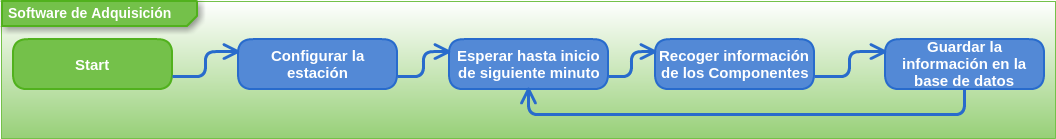
\includegraphics[keepaspectratio, width=1\textwidth]{./img/soft_control_preliminar.png}
			\caption{Software de adquisición. Diseño preliminar.}
			\label{fig:soft_control_preliminar}
		\end{figure}
	\subsection{Herramienta Web}
		En la figura \ref{fig:herramienta_web_preliminar} podemos ver el diseño preliminar de la herramienta Web. Como podemos ver el diseño
		está fuertemente basado en el patrón \emph{Modelo Vista Controlador}\cite{MVCWiki}. A continuación explicamos los tres componentes
		básicos.
		\begin{description}
			\item[Base de Datos]    
				En este componente residen los datos de nuestra estación. Para la gestión de estos utilizamos un servidor
				MySQL\cite{MySql}.
			\item[\emph{Back-End}]
				Este componente es el encargado de recibir y procesar los mensajes de petición provenientes del \emph{Front-End}.
				Estas peticiones pueden ser de consulta o de acción. En ambos casos este componente procede a comunicarse con la base
				de datos a fin de satisfacer la petición. Finalmente el resultado es trasmitido al \emph{Front-End} en un mensaje de
				respuesta. En el caso de una petición de consulta son devueltos los datos especificados. En el caso de una petición de
				acción es devuelto un mensaje de estado. Para la implementación de este componente hemos utilizado
				ZendFramework\cite{ZF} y Apygility\cite{Apigility}.
			\item[\emph{Front-end}] 
				Este componente implementa la interfaz de nuestra aplicación. Es el encargado de presentar la información y manejar
				las peticiones del usuario. El módulo está basado en el patrón MVC. Para implementar la Vista hemos utilizado
				HighStock\cite{HighStock}, para el Controlador ExtJs\cite{ExtJs} y para el modelo peticiones Ajax\cite{AjaxWiki}.
		\end{description}
		\begin{figure}[h]
			\centering
			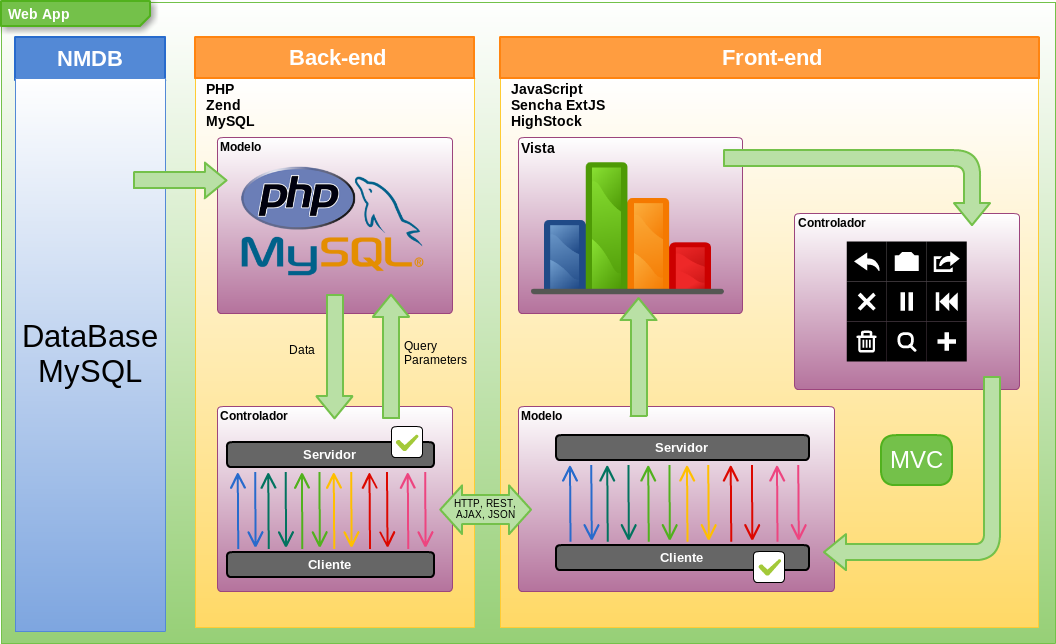
\includegraphics[keepaspectratio, width=1\textwidth]{./img/herramienta_web_preliminar.png}
			\caption{Herramienta Web. Diseño preliminar}
			\label{fig:herramienta_web_preliminar}
		\end{figure}
\section{Proceso de adquisición}
	El propósito de este punto es explicar algunos aspectos del proceso de adquisición que son relevantes para este trabajo.
	\begin{description}[leftmargin=0cm]
		\item[Múltiples Tubos]
			Hasta este momento siempre hemos hablado de tubos contadores, en plural, detrás de esto hay una razón. Normalmente las
			estaciones se componen de varios tubos contadores, donde 18 tubos contadores es un estándar. En el proceso de adquisición
			están envueltos muchos factores probabilísticos, esto conlleva a que las medidas en un tubo tengan una gran dispersión. La
			solución de este problema es tener mucho tubos, cuantos más mejor. Combinando datos de diferentes tubos conseguimos reducir
			esta dispersión. 
		\item[Valor global]
		  	Tener los datos de muchos tubos contadores permite reducir la dispersión de los datos, sin embargo no es muy práctico trabajar
			con esos datos en crudo. El software del sistema de adquisición actual calcula un valor global a partir de los datos de todos
			los tubos contadores. El software de adquisición que desarrollamos en este trabajo también debe calcular este valor global.
			Para este propósito utilizamos el Median Algorithm\cite{MedianAlgr}.
		\item[Correcciónes]
			Anteriormente en este capítulo explicamos las cascadas atmosféricas que son originadas por los rayos cósmicos. Estas cascadas
			atmosféricas dependen de la presión atmosférica. Cuando esta es elevada, es necesaria más energía para que la cascada se
			propague hasta el nivel terrestre, por consecuente los monitores de neutrones registran menos eventos. El valor de la presión
			atmosférica es monitorizado por los monitores de neutrones. Este valor es utilizado para realizar una corrección por presión
			sobre el valor global de la estación. A lo largo de este trabajo utilizamos el término de \emph{valor corregido por presión}.
			El software de adquisición elaborado para este trabajo debe ser capaz de leer el valor de presión desde un barómetro y debe
			poder calcular esta corrección. 
			\par
			También es realizada una \emph{corrección por eficiencia}. Esta es muy simple y consiste en aplicar un factor multiplicativo
			al valor corregido por presión. Este valor es utilizado para para solventar problemas técnicos. Cambios en el entorno
			inmediato del instrumento o cambios en la electrónica utilizada pueden afectan a la cantidad de eventos medidos. Estos cambios
			son identificados, evaluados y finalmente contrarrestados con esta corrección por eficiencia. Este valor dota la estación de
			consistencia histórica, de esta manera pueden ser comparados datos de diferentes intervalos temporales. El software también
			debe ser capaz de realizar esta corrección. 
		\item[Fuentes de alta tensión]
			A principios de este capítulo explicamos que los tubos contadores están rellenos de gas ionizado. Este gas es ionizado
			mediante la aplicación de una corriente eléctrica de alta tensión. Para la generación de esta corriente son utilizadas fuentes
			de alimentación de alta tensión. Cambios en la corriente generada pueden afectar a la cantidad de eventos registrados. Esto ha
			conllevado a que el funcionamiento de las fuentes sea monitorizado. El software para el sistema de adquisición debe ser capaz
			de realizas esta operación. Es de esperar que la corriente sea constante, por lo que no es necesaria ninguna corrección en
			función de esta. En caso de variaciones en la corriente los datos generados son considerados no consistentes.
		\item[\emph{Spikes}]
			Un \emph{Spike} es un dato anómalo, un dato anormalmente grande o pequeño. Son datos producidos por malfuncionamientos de la
			instrumentación, cambios bruscos en el entorno inmediato u otros factores desconocidos. Estos están presentes en todas las
			estaciones. Con la elaboración del nuevo sistema de adquisición se pretende reducir el número de \emph{Spikes} generados. Con
			la elaboración de la herramienta Web pretendemos ofrecer un método fácil de identificar y descartar dichos datos.
	\end{description}
